\section{Proof of concept}

\begin{figure}
  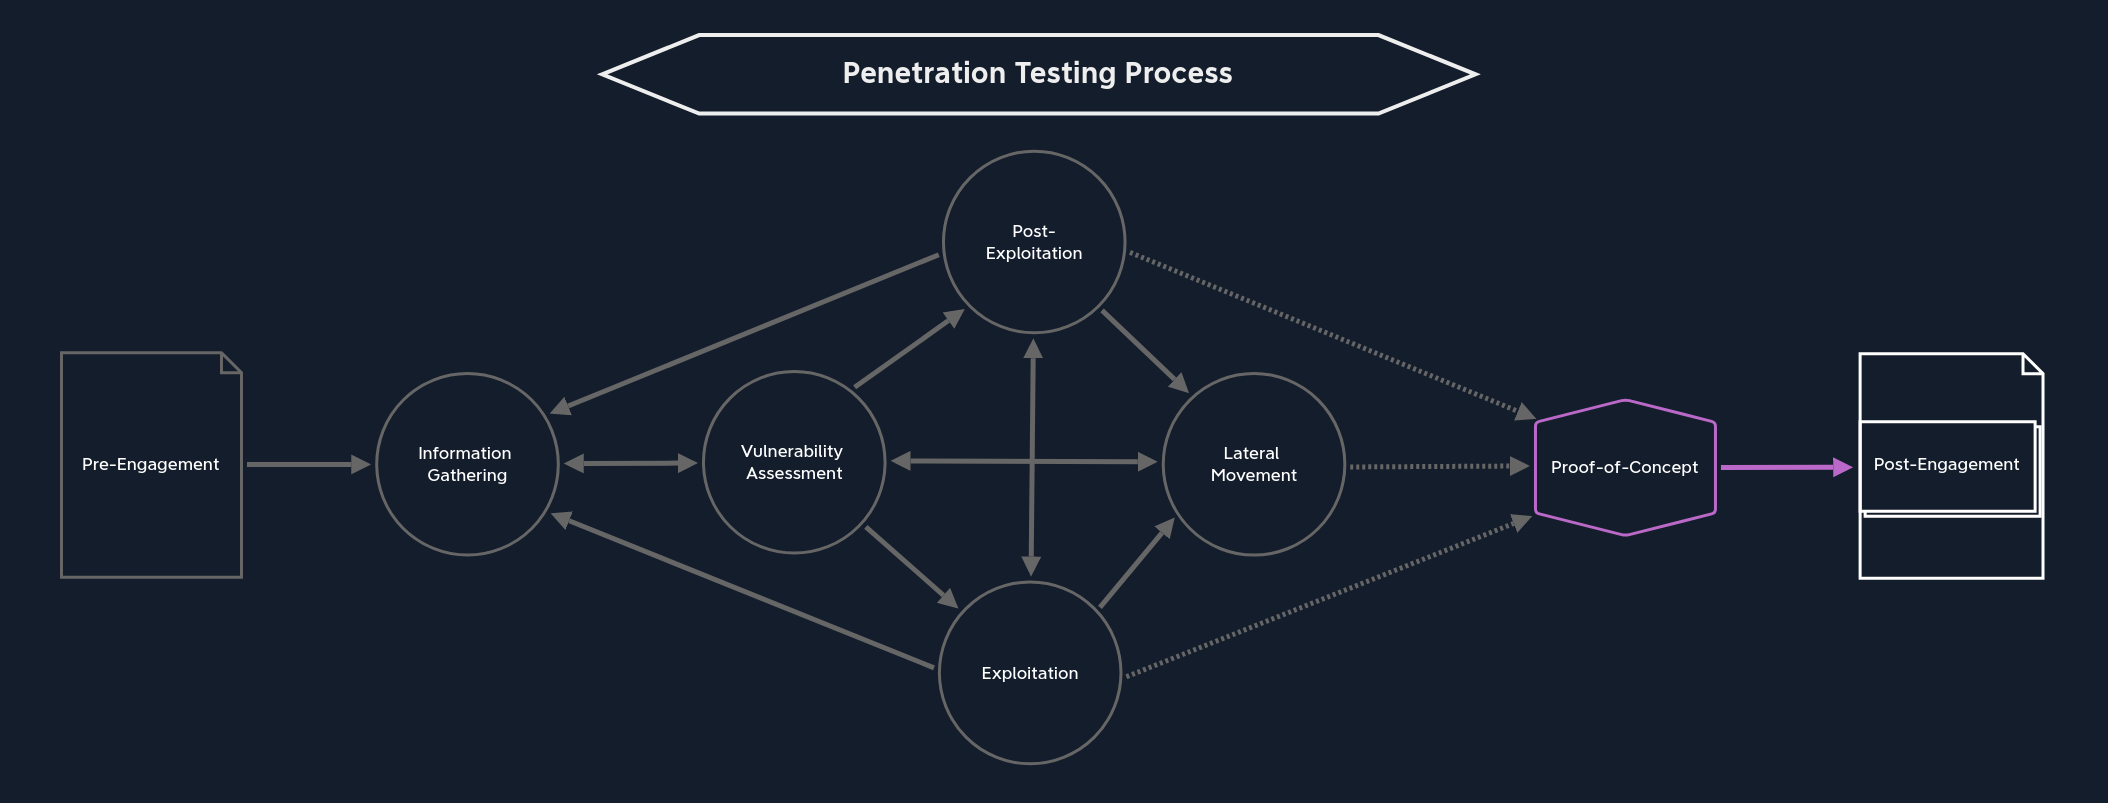
\includegraphics[width=\linewidth]{intro/process/images/poc.png}
  \caption{Proof of concept}
  \label{fig:pentest-process-poc}
\end{figure}

Proof of Concept (PoC) or Proof of Principle is a project management term. In
project management, it serves as proof that a project is feasible in principle.
The criteria for this can lie in technical or business factors. Therefore, it
is the basis for further work, in our case, the necessary steps to secure the
corporate network by confirming the discovered vulnerabilities. In other words,
it serves as a decision-making basis for the further course of action. At the
same time, it enables risks to be identified and minimized.

This project step is often integrated into the development process for new
application software (prototyping) or IT security solutions. For us in
information security, this is where we prove vulnerabilities in operating
systems or application software. We use this PoC to prove that a security
problem exists so that the developers or administrators can validate it,
reproduce it, see the impact, and test their remediation efforts. One of the
most common examples used to prove software vulnerabilities is executing the
calculator (calc.exe on Windows) on the target system. In principle, the PoC
also assesses the probability of success of system access from actual
exploitation.

A PoC can have many different representations. For example, documentation of
the vulnerabilities found can also constitute a PoC. The more practical version
of a PoC is a script or code that automatically exploits the vulnerabilities
found. This demonstrates the flawless exploitation of the vulnerabilities. This
variant is straightforward for an administrator or developer because they can
see what steps our script takes to exploit the vulnerability.

However, there is one significant disadvantage that has occurred from time to
time. Once the administrators and developers have received such a script from
us, it is easy for them to "fight" against our script. They focus on changing
the systems so that the script we created no longer works. The important thing
is that the script is only one way of exploiting a given vulnerability.
Therefore, working against our script instead of with it and modifying and
securing the systems so that our script no longer works does not mean that the
information obtained from the script cannot be obtained in another way. It is
an important aspect that should be discussed with the administrators and
developers and explicitly mentioned and pointed out.

The report they receive from us should help them see the entire picture, focus
on the broader issues, and provide clear remediation advice. Including an
attack chain walkthrough in the event of domain compromise during an internal
is a great way to show how multiple flaws can be combined and how fixing one
flaw will break the chain, but the other flaws will still exist. If these are
not also fixed, there may be another path to get to the point where the attack
chain was remediated and continue onwards. We should also drive this point home
during our report review meeting.

For example, if a user uses the password Password123, the underlying
vulnerability is not the password but the password policy. If a Domain Admin is
found to be using that password and it is changed, that one account will now
have a stronger password, but the problem of weak passwords will likely still
be endemic within the organization.

If the password policy followed high standards, the user would not be able to
use such a weak password. Administrators and developers are responsible for the
functionality and the quality of their systems and applications. Furthermore,
high quality stands for high standards, which we should emphasize through our
remediation recommendations.
